\documentclass[hyperref={pdfpagelabels=false},usepdftitle=false]{beamer}
\usepackage{../templates/myStyle}

\begin{document}
\selectlanguage{english}

\title{\titleText}
\subtitle{Bachelor's thesis of Martin Thoma}
\author{\tutor}
\date{5th of June, 2014}
%\subject{Programmieren}

\frame{\titlepage}

\frame{
    \frametitle{Contents}
    \setcounter{tocdepth}{1}
    \tableofcontents
    \setcounter{tocdepth}{2}
}

%\AtBeginSection[]{
%    \InsertToC[sections={\thesection}]  % shows only subsubsections of one subsection
%}

\section{What is my Bachelor's thesis about?}
%!TEX root = Sommerakademie-2015-Forschung.tex
\section{Einleitung}
\subsection{Was ist On-Line Recognition?}

\begin{frame}{Demo}
    \begin{figure}[h]
        \centering
        \includegraphics*[width=0.7\linewidth, keepaspectratio]{images/Classification.png}
    \end{figure}

    \href{http://write-math.com}{write-math.com}
\end{frame}

\begin{frame}{Was ist On-Line Recognition?}
\medskip
\begin{columns}[t,onlytextwidth]
\begin{column}{.5\textwidth}
{\Large Off-line Recognition}
\begin{figure}[h]
    \centering
    \includegraphics*[width=0.7\linewidth, keepaspectratio]{images/A-pixel.png}
\end{figure}
\end{column}
\begin{column}{.5\textwidth}
{\Large On-line Recognition}
\begin{figure}[h]
    \centering
    \includegraphics*[width=0.7\linewidth, keepaspectratio]{images/A-vektor.png}
\end{figure}
\end{column}
\end{columns}
\end{frame}

\begin{frame}{Was wollen wir?}
    \[f(\text{Merkmale}) = \begin{pmatrix}0.7\\ 0.1\\ 0.2\end{pmatrix} = \begin{pmatrix} \mathbb{P}(\gamma)\\ \mathbb{P}(\text{ö})\\ \mathbb{P}(\heartsuit) \end{pmatrix}\]
    \medskip
    \visible<2->{
        \begin{center}
        {\Large Gesucht: Funktion $f$}\\
        (und Merkmalsextraktion)
    }
    \end{center}
\end{frame}

\begin{frame}{Merkmalsextraktion}
    \begin{figure}[h]
        \centering
        \includegraphics*[width=0.7\linewidth, keepaspectratio]{images/A-vektor-merkmalsbildung.png}
    \end{figure}

    Merkmalsvektor fester Länge ist praktisch
\end{frame}

\section{Funktionen}
\subsection{Funktionen}

\begin{frame}{Funktionen}
\begin{figure}[h]
    \centering
    \includegraphics*[width=0.7\linewidth, keepaspectratio]{images/function-machine.png}
\end{figure}
\end{frame}
\begin{frame}{Funktionen}
    \medskip
    \begin{columns}[t,onlytextwidth]
    \begin{column}{.5\textwidth}{
        \begin{itemize}[<+->]
            \item $f(x) = x^2$ ist $f: \mathbb{R} \rightarrow \mathbb{R}$
            \item $f(x, y) = x^2 + y^2$ ist $f: \mathbb{R}^2 \rightarrow \mathbb{R}$
            \item $f(x, y) = (x^2 + y^2, x \cdot y)$ ist $f: \mathbb{R}^2 \rightarrow \mathbb{R}^2$
        \end{itemize}
    }
    \end{column}
    \begin{column}{.4\textwidth}
    \only<1>{
        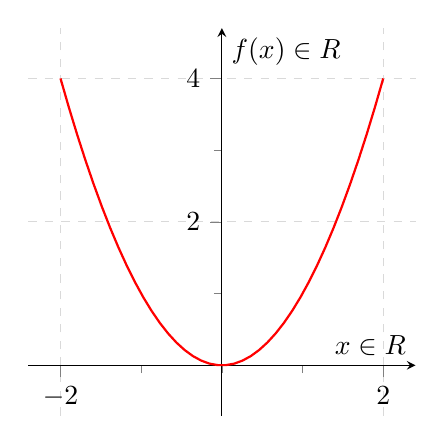
\begin{tikzpicture}
            \begin{axis}[
                legend pos=south west,
                axis x line=middle,
                axis y line=middle,
                grid = major,
                width=6.5cm,
                height=6.5cm,
                grid style={dashed, gray!30},
                xmin=-2,     % start the diagram at this x-coordinate
                xmax= 2,     % end   the diagram at this x-coordinate
                ymin=-0.25,  % start the diagram at this y-coordinate
                ymax= 4.25,  % end   the diagram at this y-coordinate
                axis background/.style={fill=white},
                xlabel=$x \in \mathbb{R}$,
                ylabel=$f(x) \in \mathbb{R}$,
                %xticklabels={-2,-1.6,...,7},
                %yticklabels={-8,-7,...,8},
                tick align=outside,
                minor tick num=-3,
                enlargelimits=true,
                tension=0.08]
              \addplot[domain=-2:2, red, thick,samples=40] {x*x};
            \end{axis}
        \end{tikzpicture}
    }
    \only<2->{
        \pgfplotsset{
            colormap={whitered}{
                color(0cm)=(white);
                color(1cm)=(orange!75!red)
            }
        }
        \begin{tikzpicture}
            \begin{axis}[
            colormap name=whitered,
            width=5.5cm,
            height=5.5cm,
            view={340}{25},
            enlargelimits=false,
            grid=major,
            domain=-3:3,
            y domain=-3:3,
            samples=56, %57 : TeX capacity exceeded, sorry [main memory size=3000000].
                        % see also http://tex.stackexchange.com/a/7954/5645
            xlabel=$x$,
            ylabel=$y$,
            zlabel={$f(x,y)$},
            ]
              \addplot3[surf] {x^2 + y^2};
            \end{axis}
        \end{tikzpicture}
    }
    \end{column}
    \end{columns}
\end{frame}

\begin{frame}{Funktionen mit Parametern}
    \begin{columns}
    \begin{column}{.5\textwidth}
        {\Large Mit Parametern}
        \begin{itemize}[<+->]
            \item $f(x) = x^2$
            \item $f(x) = 2 \cdot x^2$
            \item $f(x) = \nicefrac{1}{2} \cdot x^2$
            \item $f(x) = a \cdot x^2$
            \item $f(x_1, \dots, x_{166}) = \sum_{i=1}^{166} a_i \cdot x_i$\\
                  $\mathbb{R}^{166} \rightarrow \mathbb{R}$
            \item $f(x_1, \dots, x_{166}) = (\sum_{i=1}^{166} a_i \cdot x_i, \dots, \sum_{i=1}^{166} z_i \cdot x_i)$\\
                  $\mathbb{R}^{166} \rightarrow \mathbb{R}^{\text(\# Klassen)}$
        \end{itemize}
    \end{column}
    \begin{column}{.4\textwidth}
        \begin{tikzpicture}
            \begin{axis}[
                legend pos=south west,
                axis x line=middle,
                axis y line=middle,
                grid = major,
                width=6.5cm,
                height=6.5cm,
                grid style={dashed, gray!30},
                xmin=-2,     % start the diagram at this x-coordinate
                xmax= 2,     % end   the diagram at this x-coordinate
                ymin=-0.25,  % start the diagram at this y-coordinate
                ymax= 4.25,  % end   the diagram at this y-coordinate
                axis background/.style={fill=white},
                xlabel=$x \in \mathbb{R}$,
                ylabel=$f(x) \in \mathbb{R}$,
                %xticklabels={-2,-1.6,...,7},
                %yticklabels={-8,-7,...,8},
                tick align=outside,
                minor tick num=-3,
                enlargelimits=true,
                tension=0.08]
              \only<1->{\addplot[domain=-2:2, red, thick,samples=40] {x*x};}
              \only<2->{\addplot[domain=-2:2, blue, thick,samples=40] {2*x*x};}
              \only<3->{\addplot[domain=-2:2, green, thick,samples=40] {0.5*x*x};}
            \end{axis}
        \end{tikzpicture}
    \end{column}
    \end{columns}
\end{frame}

\begin{frame}{Fehlerfunktion}
    \begin{itemize}[<+->]
        \item \textbf{Daten $(x_{i,1}, \dots, x_{i,n}, y_{i,1}, \dots, y_{i,\text{\# Klassen}})$}: Beispiele für den Computer
        \item \textbf{Aktuelles Modell $f$}: Funktion mit vielen Parametern
        \item \textbf{Fehlerfunktion}: Wie gut ist $f$ für die vorhandenen
              Daten?
    \end{itemize}
\end{frame}

\begin{frame}{Fehlerfunktion}
    Abbildung von \textbf{Parameterraum} auf den Fehler ($\mathbb{R}_0^+$)
\end{frame}

\begin{frame}{Minimieren mit Ableitungen}
    \begin{figure}[h]
        \centering
        \includegraphics*[width=0.7\linewidth, keepaspectratio]{images/derivative-function.png}
    \end{figure}
\end{frame}

\begin{frame}{Gradientenabstieg}
    \begin{figure}[h]
        \centering
        \includegraphics*[width=0.7\linewidth, keepaspectratio]{images/gradient-descent.png}
    \end{figure}
\end{frame}


\section{Neuronale Netze}
\subsection{Neuronale Netze}
\begin{frame}{Neuronale Netze}{}
    \begin{itemize}[<+->]
        \item Menge von parametrisierten Funktionen
              $\mathbb{R}^n \rightarrow \mathbb{R}^{\text(\# Klassen)}$
        \item $\mathbb{R}^n$: Eingabe,\\z.B. Farbe von Pixel~1, Farbe von Pixel~2, \dots
        \item $\mathbb{R}^{\text(\# Klassen)}$: Ausgabe,\\Wahrscheinlichkeit der Klasse (z.B. 0, 1, 2, 3, 4, 5, 6, 7, 8, 9)
        \item Ableitbar
    \end{itemize}
\end{frame}

\section{Ausblick}
\subsection{Ausblick}
\begin{frame}{Ausblick}
    Erkennung von Formeln
    \begin{itemize}[<+->]
        \item Aufbau eines Sprachmodells der Mathematik
        \item Erweiterung der Symboldatenbank
        \item Segmentierung
    \end{itemize}
\end{frame}



\section{write-math.com}
\subsection{Write Math}

\begin{frame}{write-math.com}
    \begin{itemize}
        \item a website where users can add labeled training data and unlabeled
              data which they want to classify. I call this data \enquote{recording}
        \begin{figure}[ht]
            \centering
            \subfloat{
                
\includegraphics[height=0.1\textwidth]{../images/279952.pdf}
            }%
            \qquad
            \subfloat{
                
\includegraphics[height=0.1\textwidth]{../images/281507.pdf}
            }%
            \qquad
            \subfloat{
                
\includegraphics[height=0.1\textwidth]{../images/287612.pdf}
            }%
            \qquad
            \subfloat{
                
\includegraphics[height=0.1\textwidth]{../images/292175.pdf}
            }%
            \caption*{4 recordings}
        \end{figure}
        \item works with desktop computers and touch devices
        \item symbol recognition can be done by multiple classifiers
        \item users can contribute formulas as recordings and as \LaTeX{} answers
              for recordings
        \item users can vote for \LaTeX{} answers:
              \Large $\leq$, $\leqq$, $\leqslant$, \dots \normalsize
        \item user who entered the recording can accept one answer
    \end{itemize}
\end{frame}

\framedgraphic{Classify}{../images/classify.png}
\framedgraphic{Workflow}{../images/workflow.png}
% \framedgraphic{User page}{../images/user-page.png}
% \framedgraphic{Information about recordings}{../images/view.png}
% \framedgraphic{Symbol page}{../images/symbol.png}
% \framedgraphic{Training}{../images/train.png}
\framedgraphic{Ranking}{../images/ranking.png}


\begin{frame}[fragile]{Statistics}
    \begin{itemize}
        \item 127 users with at least 5 recordings
        \item $\num{1111}$ symbols, but only $\num{369}$ used for experiments
        \item $\num{235831}$ recordings (e.g. $\num{3489}$ times \verb+\int+, but only 50 times \verb+X+)
    \end{itemize}
\end{frame}

\begin{frame}{First classification worker}
    \begin{itemize}
        \item preprocessing: Scale to fit into unit square while keeping the aspect
              ratio
        \item applies greedy time warping
        \item compares a new recording with every recording
              in the database
        \item[$\Rightarrow$] Classification time is in $\mathcal{O}(\text{recordings})$,
              but we rather would like $\mathcal{O}(\text{symbols})$
        \item the current server / workflow can only handle about 4000 recordings
        \item[$\Rightarrow$] Another way to classify is necessary
    \end{itemize}
\end{frame}

\section{Preprocessing and Features}
\subsection{Preprocessing}
\begin{frame}{Preprocessing}
    \begin{itemize}
        \item Normalizing
        \begin{itemize}
            \item Scaling
            \item Shifting
            \item Resampling
        \end{itemize}
        \item Noise reduction
        \begin{itemize}
            \item Smoothing (e.g. moving average)
            \item Dot reduction
            \item Filtering (by distance, speed or angle)
            \item Stroke connection
        \end{itemize}
    \end{itemize}
\end{frame}
\subsection{Features}
\begin{frame}{Features}
    \begin{itemize}
        \item Local
        \begin{itemize}
            \item Coordinates
            \item Speed
            \item Binary pen pressure
            \item Direction
            \item Curvature
            \item Bitmap-environment
            \item Hat-Feature
        \end{itemize}
        \item Global
        \begin{itemize}
            \item \# of points
            \item \# of strokes
            \item Center point
            \item Bitmap
            \item Bounding box (width, height, time)
        \end{itemize}
    \end{itemize}
\end{frame}

\section{Neural Nets}
\subsection{Neural Net experiments}
\begin{frame}{Experiments}
    \textbf{Preprocessing:} Scaling, shifting and linear interpolation\\
    \textbf{Features:} Coordinates of 80 points (4 strokes with 20 points each)\\
    \textbf{Learning:} MLP, 300 epochs, LR of 0.1, Momentum 0.1

\begin{table}[h]
    \begin{tabular}{lrl}
    \toprule
    Topology                & Error    & Training time \\ \midrule
    160:500:369             & 30.62 \% & \hphantom{0}9min 08s      \\
    160:500:500:369         & 27.73 \% & 11min 49s     \\
    160:500:500:500:369     & 34.79 \% & 14min 09s     \\
    160:500:500:500:500:369 & 33.61 \% & 14min 06s     \\
    \bottomrule
    \end{tabular}
\end{table}

\end{frame}

\begin{frame}[fragile]{Examples of confusable symbols}
\begin{table}[ht]
    \centering
    \begin{tabular}{lc|lc}
        \textbf{\LaTeX}& \textbf{Rendered}   & \textbf{\LaTeX}& \textbf{Rendered} \\\midrule
        \verb+\sum+    & $\sum$         & \verb+$\Sigma$+        & $\Sigma$\\
        \verb+\coprod+ & $\coprod$      & \verb+$\amalg$+        & $\amalg$\\
        \verb+\perp+   & $\perp$        & \verb+$\bot$+          & $\bot$\\
        \verb+\models+ & $\models$      & \verb+$\vDash$+        & $\vDash$\\
        \verb+\emptyset+ & $\emptyset$  & \verb+$\diameter$+     & $\diameter$\\
        ~              & ~              & \verb+$\o$+            & $\o$\\
        ~              & ~              & \verb+$\varnothing$+   & $\varnothing$\\
        \verb+\Delta+  & $\Delta$       & \verb+$\triangle$+     & $\triangle$\\
        \verb+\varepsilon+ & $\varepsilon$ & \verb+$\mathcal{E}$+ & $\mathcal{E}$\\
    \end{tabular}
\end{table}

When those confusions are not counted as errors, the current best system
has an classification error rate of $12.7 \%$ (otherwise $22.2 \%$).

\end{frame}

\section{What will I do next?}
\subsection{What will I do next?}
\begin{frame}{What will I do next?}
    \begin{itemize}
        \item Include the currently best model in write-math.com
        \item Evaluate preprocessing steps
        \item Try other features
        \item Try other topologies / trainings (e.g. pretraining, newbob)
        \item Eventually try convolutional neural nets
    \end{itemize}
\end{frame}

% \subsection{Far future}
% \begin{frame}{What could be done?}
%     \begin{itemize}
%         \item Make use of audio data in a multimodal approach\\
%               e.g. $R$ and $\mathcal{R}$
%         \item Currently, the Lecture Translation system doesn't recognize math.\\
%               You get \enquote{integral of e raised to the power of x d x} instead
%               of $\int e^x \mathrm{d} x$.
%         \item Spoken math is ambigous: $\sqrt{a+b}$ vs. $\sqrt{a} + b$
%         \item The language model I create could help to find probable formulas
%         \item The platform could be used to get more input data of users
%     \end{itemize}
% \end{frame}

\section*{End}
\subsection{End}
\subsection{Sources}
\begin{frame}{Image Sources}
    \begin{itemize}
	\item \href{https://commons.wikimedia.org/wiki/File:Server-multiple.svg}{Server} by RRZEicons
    \item \href{https://commons.wikimedia.org/wiki/File:Computer-aj_aj_ashton_01.svg}{Desktop Computer} by Ed g2s,
          Ironbrother, Kierancassel and Msgj
    \item \href{https://commons.wikimedia.org/wiki/File:Server_by_mimooh.svg}{Server} by Mimooh
    \end{itemize}

    The presentation can be found at \url{http://tinyurl.com/write-math-short-presentation}
\end{frame}


\framedgraphic{Thanks for Your Attention!}{../images/xi.png}

\end{document}
